% vim: tw=78 encoding=utf8 ts=2 sw=2 expandtab softtabstop=2
\documentclass[11pt,twocolumn,a4paper,english]{article}

\usepackage[utf8]{inputenc}
\usepackage{babel}
\usepackage{url}
\usepackage{graphicx}
\usepackage{anysize}
\marginsize{1.7cm}{1.7cm}{1.7cm}{1.7cm}

\newcommand{\TODO}{\textbf{TODO:} }

\title{
Synthesizing Benchmarks for Architecture Recovery Algorithms}
\author{Rodrigo Souza \\ rodrigorgs@gmail.com 
\and Dalton Guerrero \\ dalton@dsc.ufcg.edu.br
\and Jorge Figueiredo \\ abrantes@dsc.ufcg.edu.br
\and Christina Chavez \\ flach@ufba.br
}

\begin{document}

\sloppy
\maketitle

\begin{abstract}
	As a software system evolves, its actual architecture may deviate from its original reference architecture. A better understanding of the actual architecture can be gained by applying architecture recovery algorithms to the source code of the system. Unfortunately, there is little knowledge regarding the quality of such algorithms, mostly because, in order to assess their accuracy, one needs updated, detailed architectures for a variety of software systems.
	To overcome such problem, we propose a simulation model that synthesizes implementation-level dependency graphs that conform to the module view of any given reference architecture. We show, using observations from network theory, that the graphs are very similar to dependency graphs extracted from the source code of real software systems. 
	Then, we synthesize thousands of graphs, in a controlled way, and use them as benchmarks for six well-known architecture recovery algorithms: ACDC, Bunch, SL75, SL90, CL75, and CL90. By comparing the given reference architectures with those recovered by the algorithms, we conclude that ACDC and Bunch outperform the alternatives, specially if the architecture contains more than a couple of modules.\end{abstract}

%%%%%%%%%%%%%%%%%%%%%%%%%%%%%%%%%%%%%%%%%%%%%%%%%%%%%%%%%%%%%%%%%%%%%%%%%%%%%
%%%%%%%%%%%%%%%%%%%%%%%%%%%%%%%%%%%%%%%%%%%%%%%%%%%%%%%%%%%%%%%%%%%%%%%%%%%%%

% I use begin/end instead of just \section so I can fold sections in my text editor
\begin{section}{Introduction}
% This section should be succinct, with no subheadings
	Architectural drift

	Reverse engineering / Architecture recovery algorithms
	
\end{section}

%%%%%%%%%%%%%%%%%%%%%%%%%%%%%%%%%%%%%%%%%%%%%%%%%%%%%%%%%%%%%%%%%%%%%%%%%%%%%

\begin{section}{Background}
	Architecture recovery algorithms

	Evaluation of architecture recovery algorithms. 
	
\end{section}

%%%%%%%%%%%%%%%%%%%%%%%%%%%%%%%%%%%%%%%%%%%%%%%%%%%%%%%%%%%%%%%%%%%%%%%%%%%%%

\begin{section}{The BCR+ model}	
	\newcommand{\din}[0]{\ensuremath{\delta_{in}}}
	\newcommand{\dout}[0]{\ensuremath{\delta_{out}}}
	\newcommand{\gin}[0]{\ensuremath{\mathrm{g}_{in}}}
	\newcommand{\gout}[0]{\ensuremath{\mathrm{g}_{out}}}
	
	\TODO Talk about network theory / complex networks / scale-free networks	

	When designing the architecture of a software system, the module viewpoint plays a major role, by specifying the modules of the system and their inter-relationships. Constraining such dependencies benefits the maintenatibility, portability, and reusability of the software system.
	
	In this section, we describe the BCR+ model for synthesizing graphs from a description of the module viewpoint of an arbitrary architecture --- that is, the modules and dependencies between modules. The BCR+ model produces---by means of the mechanisms of growth and preferential attachment---directed graphs that are both scale-free and segmented in modules.
	
	\TODO there are other models, but they don't take architecture as input	
	
\begin{subsection}{Overview}
	The BCR+ model is a generalization of a graph model proposed by Bollobás et al \cite{Bollobas2003}. The original model generates directed graphs that are scale-free. Our model extends the original by generating graphs in which the nodes are organized in modules, according to an modular architecture given as input.
	
	The BCR+ model takes the following parameters as input:
	
	\begin{itemize}
  \item number of vertices, $n$;
  \item three probability values, $p_1$, $p_2$ e $p_3$, com $p_1 + p_2 + p_3 = 1$;
  \item base in-degree, $\din$;
  \item base out-degree, $\dout$.
  \item an directed graph representing dependencies between modules, $G$;
  \item a constant, $\mu$, with $0,0 \le \mu \le 1,0$;
  \end{itemize}
  
	The last two parameters are new in BCR+. The other ones are from the original model by Bollobás et al \cite{Bollobas2003}.
	
	In the graph $G$, each vertex represents one module of the architecture. Each edge defines a relationship of dependency between modules. We say that a module $M_1$ depends on another module, $M_2$, if $G$ contains an edge from the vertex that represents $M_1$ to the vertex that represents $M_2$. In the graph that is created, an edge from a vertex $v_1 \in M_1$ to another vertex, $v_2 \in M_2$, can be created only if $M_1$ depends on $M_2$ in the graph $G$ or if $M_1$ and $M_2$ are the same module.
	
		\TODO Say that these graphs contain both internal and external edges. Define internal/external.
		
	The parameter $\mu$ controls the proportion of external edges in the graph---that is, edges connecting vertices in distinct modules. Lower values lead to graphs with fewer external edges.
	
	The original model by Bollobás et al \cite{Bollobas2003} is a particular case of BCR+ when $\mu = 0$ and $G$ contains one single vertex, representing one single module.
	

\begin{figure*}[htbp]
	\centering
		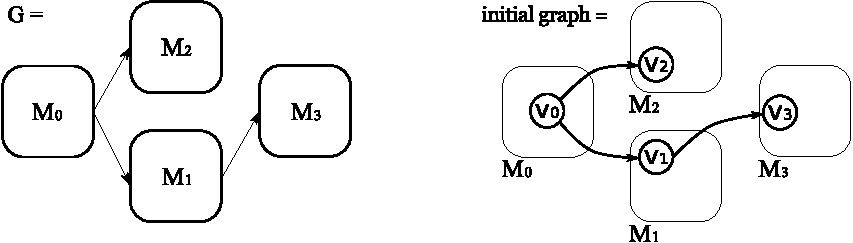
\includegraphics[scale=1]{figures/bcr-initial-graph}
	\caption{Initial graph synthesized by BCR+, given an input graph parameter $G$.}
	\label{fig:bcr-initial-graph}
\end{figure*}
	
	As a computer model, BCR+ takes the parameters as inputs and, by running an algorithm, outputs a graph. The algorithm builds the output graph incrementally. It starts by creating a module for each vertex in the input graph $G$, and then adding one vertex to each module. After that, it creates all external edges that are allowed by $G$ (see Figure \ref{fig:bcr-initial-graph}). Then, the graph is modified according to three formation rules that are applied successively, in random order, until the graph grows to $n$ vertices. At each algorithm step, the probability of the $i$-th being applied is given by the parameter $p_i$.

\end{subsection}	

\begin{subsection}{Formation Rules}
	
	There are three formation rules in BCR+. Each one modifies the output graph by adding or removing vertices or edges in the graph. Also, each formation rule has a probability of being applied, given by the parameters $p_1$, $p_2$ and $p_3$.

\begin{figure*}[htbp]
	\centering
		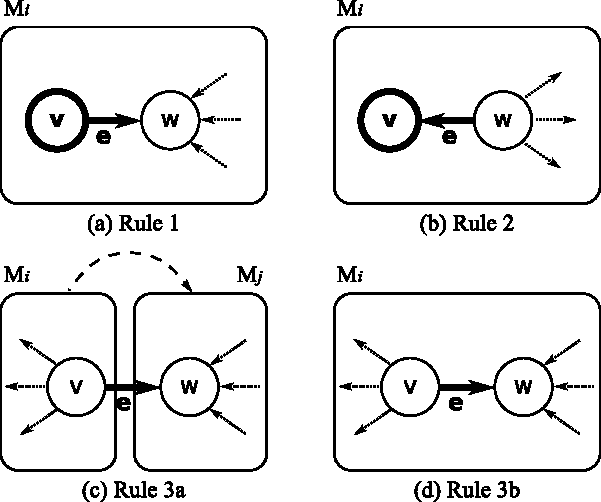
\includegraphics[scale=1]{figures/bcr-rules}
	\caption{Formation rules for BCR+. $M_i$ and $M_j$ are distinct modules, such as $M_i$ depends on $M_j$. In the diagram for each rule, thicker lines represent vertices and edges created when the rule is applied.}
	\label{fig:bcr-rules}
\end{figure*}

	The rules are illustrated in Figure \ref{fig:bcr-rules}. Simplified rules:
	
	\begin{itemize}
		\item Rule 1: one vertex is added to some module, together with an outgoing edge to another vertex in the same module.
		\item Rule 2: one vertex is added to some module, together with an ingoing edge coming from another vertex in the same module.
		\item Rule 3: one edge is added between two pre-existing vertices. There are two variations of this rule:
		\begin{itemize}
			\item Rule 3a: choose vertices from distinct modules.
			\item Rule 3b: choose vertices that are in the same module.
		\end{itemize}
	\end{itemize}
	
	The rules 1, 2, and 3b come directly from the original model by Bollobás et al \cite{Bollobas2003}. The rule 3a was created in BCR+ to account for inter-module dependencies.
	
	The choice of vertices to which add edges to is done according to preferential attachment. When we say that a vertex ``chosen according to $\mathrm{f}(x)$'', we mean that the probability of choosing the vertex $x$ is proportional to $\mathrm{f}(x)$:
	
	$$
	  \mathrm{P}(x) ~=~ \frac{ \mathrm{f}(x) }
	  { \displaystyle\sum_{i} \mathrm{f}(i) }
	$$
	
	The denominator is a normalization factor, such as the sum of probabilities $\mathrm{P}(x)$ is 1.
	
	With this definition in mind, the rules can be fully specified:
	
	\begin{itemize}
		\item Rule 1: \emph{Add a vertex with an outgoing edge}. An existing vertex, $w$, is chosen according to $\mathrm{f}(x) = \din + \gin(x)$ (that is, parameter $\din$ added to the vertex in-degree). A new vertex, $v$, is added to the module that contains $w$, together with an edge from $v$ to $w$.

		\item Rule 2: \emph{Add a vertex with an ingoing edge}. An existing vertex, $w$, is chosen according to $\mathrm{f}(x) = \dout + \gout(x)$. A new vertex, $v$, is added to the module that contains $w$, together with an edge from $w$ to $v$.

		\item Rule 3: \emph{Add an edge between pre-existing vertices}. A vertex, $v$, is chosen according to $\mathrm{f}(x) = \dout + \gout(x)$. Then, an edge is added from $v$ to another vertex, $w$, chosen according to $\mathrm{f}(x) = \din + \gin(x)$. The vertex $w$ is not chosen among the set of all vertices. In fact, there are two rules, and the choice of the rule to apply is probabilistic and depends on the parameter $\mu$:

		\begin{itemize}
		  \item Rule 3a: with proability $\mu$, $w$ is chosen among the vertices that are in modules on which the module of $v$ depends, according to the parameter $G$.
		  \item Rule 3b: with probability $1 - \mu$, $w$ is chosen among the vertices that are in the same module as $v$.
		\end{itemize}
	\end{itemize}
	
	\TODO BCR+ is a growth model, can simulate the evolution of a software system subject to constraints in module interaction. See CSMR paper (extended version), pg 2, col 2, just before section B. 
	
\end{subsection}

\begin{subsection}{Example}
	\TODO Do we need an Example section?
\end{subsection}
	
\end{section}

%%%%%%%%%%%%%%%%%%%%%%%%%%%%%%%%%%%%%%%%%%%%%%%%%%%%%%%%%%%%%%%%%%%%%%%%%%%%%

\begin{section}{Software-Realism}
	% Motifs / Triads. Triad concentration profiles.
	% Software-realism metric.
	% Software-realism classifier. Training and testing the classifier.
	% Software-realism for the BCR+ model. (Cite previous paper, where we also evaluate software-realism for three other models)
	
	If synthetic graphs are to be used as surrogates to dependency graphs extracted from the source code of software systems, it is expected that they resemble such graphs. To capture this software quality of a graph, we define the concept of software-realism, that indicates to what extent a graph resembles software dependency graphs.
	
	A metric for software-realism should be consistent, that is, it should present high values when measuring dependency graphs, and low values when measuring graphs from other domains---e.g., protein interaction networks, social networks etc.
	
	First, we define a metric for software-realism, based on structural properties of a graph. Then, we show that the metric is consistent, by applying both to software dependency graphs and to graphs from non-software domains. Finally, we show that the BCR+ model is capable of synthesizing graphs with a high degree of software-realism.
	
\begin{subsection}{Background}

	Given three vertices, one can conceive 13 distinct connected directed graphs---the so-called triads---, as shown in Figure \ref{fig:triads}. By counting how often each triad appears in a graph, one can build a vector, called triad concentration profile, that summarizes any graph in a compact, fixed-size way.

	\begin{figure*}[htbp]
		\centering
			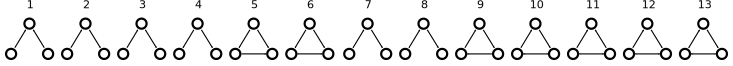
\includegraphics[scale=1]{figures/triads}
		\caption{All triads---connected directed graphs with three vertices---, numbered from 1 to 13.}
		\label{fig:triads}
	\end{figure*}
	
	Previous work has shown that graphs from the same domain tend to be caracterized by similar triad concentration profiles \cite{Milo2002}. For example, Figure \ref{fig:triads}(a) presents triad concentration profiles for two software dependency graphs, whereas Figure \ref{fig:triads}(b) presents triad concentration profiles for graphs in distinct domains: a software dependency graph and a linguistic graph. An informal analysis reveals that the similarity between the profiles is greater in the first case. It should suffice to notice that, in the second case, the concentration of the first two triads is somewhat reversed (in the linguistic graph, the second triad is the most frequent).

	\begin{figure*}[htbp]
		\centering
			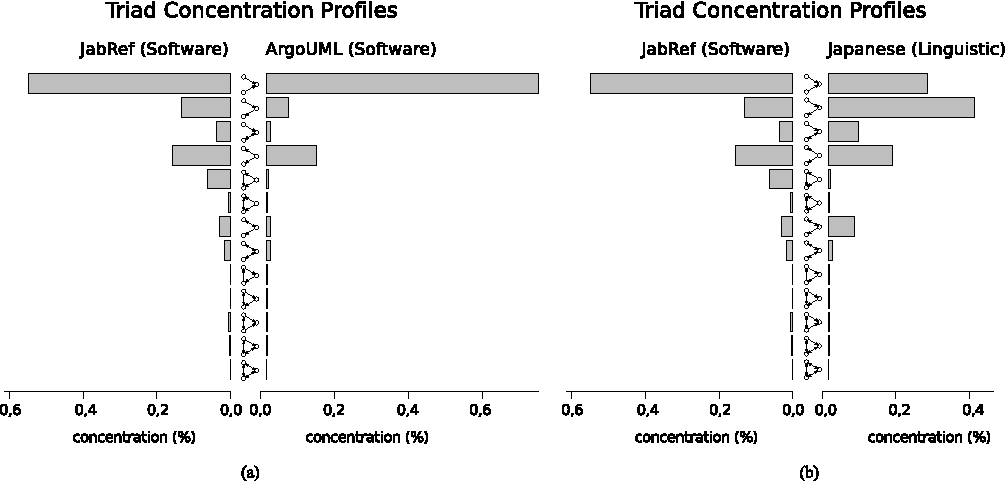
\includegraphics[scale=1]{figures/tcp}
		\caption{Comparison between triad concentration profiles for three distinct graphs (computed with the igraph tool \cite{igraph}). (a) Class dependency graphs for two softwares: JabRef, version 2.5b2 (left) and ArgoUML version 0.28 (right). (b) Graph for JabRef, version 2.5b2 (left), and graph of word succession in a sample of Japanese texts (right) \cite{Milo2004}.}
		\label{fig:tcp}
	\end{figure*}
	
	Previous works \cite{Milo2004,Ma2007,Lin2008} have explored the use of Pearson's correlation coefficient on triad concentration profiles in order to find clusters of structurally similar graphs. The results suggest that the technique is effective in identifying groups of graphs from the same domain (e.g., social, linguistic, biologic etc.).
			
	\end{subsection}
	
\begin{subsection}{Software-Realism Metric}
	
	
	\TODO Similarity between graphs:
	
	$$
  \mathrm{sim}(a, b) ~=~ 
    \mathrm{cor}(\mathrm{PCT}(a), \mathrm{PCT}(b))\mathrm{.}
  $$
	
	
	\TODO Software-realism metric:
	
	$$
  \mathrm{S}(x, R) ~=~ \frac{
  \displaystyle\sum_{s \in R} \mathrm{sim}(x, s)
  }{|R|} \mbox{.}
  $$

\end{subsection}
	
\begin{subsection}{Metric Evaluation}
	
	\TODO Classification model:
	
	$$
	  \mathrm{m}(x, R, S_0) ~=~
	  \left\{
	  \begin{array}{cl}
	  \mbox{sw-realistic,} & \mbox{se } \mathrm{S}(x, R) \ge S_0; \\
	  \mbox{non sw-realistic,} & \mbox{caso contrário.}
	  \end{array}
	  \right.
	$$	
	
	\TODO data collection; data processing (extracting dependency graphs); analysis (accuracy, precision, recall)
	
	\TODO choice of $S_0$.
	
\end{subsection}
	
\begin{subsection}{Software-Realism of BCR+}
	\TODO choice of parameters; graph synthesizing; graph classification (according to sw-realism)
\end{subsection}
	
\end{section}

%%%%%%%%%%%%%%%%%%%%%%%%%%%%%%%%%%%%%%%%%%%%%%%%%%%%%%%%%%%%%%%%%%%%%%%%%%%%%

\begin{section}{Evaluation of Architecture Recovery Algorithms}
	\TODO Traditional experimental setup for evaluation of architecture recovery algorithms: given a dependency graph and a reference architecture, run the algorithm on the graph and compare the recovered architecture with the reference architecture.
	\TODO MoJo metric.
	
	\TODO Experiment 1: comparison between arch recovery algorithms
	\TODO Experiment 2: analysis of parameters
	\TODO Experiment 3: two-way vs. one-way dependencies
\end{section}

%%%%%%%%%%%%%%%%%%%%%%%%%%%%%%%%%%%%%%%%%%%%%%%%%%%%%%%%%%%%%%%%%%%%%%%%%%%%%

\begin{section}{TODO: Other Possible Sections}
	Discussion
	
	Limitations
	
	Conclusion
	
	Acknowledgments
	
	References	
\end{section}

%%%%%%%%%%%%%%%%%%%%%%%%%%%%%%%%%%%%%%%%%%%%%%%%%%%%%%%%%%%%%%%%%%%%%%%%%%%%%
%%%%%%%%%%%%%%%%%%%%%%%%%%%%%%%%%%%%%%%%%%%%%%%%%%%%%%%%%%%%%%%%%%%%%%%%%%%%%

\bibliographystyle{plain}
\bibliography{ase2012-reference-arch}

\end{document}
